\documentclass[11pt,a4paper]{ivoa}
\input tthdefs

\lstloadlanguages{SQL}
\lstset{flexiblecolumns=true,basicstyle=\ttfamily,showstringspaces=False}
\usepackage{todonotes}

\title{Group Membership Service}

\ivoagroup{Grid and Web Services}

\author{Brian Major}
\author{Patrick Dowler}
\author{Giuliano Taffoni}
\author{Sonia Zorba}
\author{Adrian Damian}
\author{Sara Bertocco}
\author{Marco Molinaro}

\editor{Brian Major}

% \previousversion[????URL????]{????Funny Label????}
\previousversion{This is the first public release}

\begin{document}
\begin{abstract}

The Group Membership Service (GMS) specification describes a service interface for determining whether a user is a member of a group.  Membership information can be used to protect access to proprietary resources.  When an authorization decision is needed (whether to grant or deny access to a proprietary resource), a call to GMS can be made to see if the requesting user is a member of the group assigned to protect the resource in question.  Examples of proprietary resources are wide ranging but include: observation data and metadata and scarce or limited services and infrastructure.  Because this specification details how a single group can protect multiple, potentially distributed, resources, it allows for the representation of teams with common authorization rights.  The members of such teams can span multiple organizations but can be managed within a single service.  In this way, GMS offers an interoperable, flexible, and scalable mechanism for sharing proprietary assets with a potentially dynamic set of team members.

\end{abstract}

\section*{Acknowledgments}
For the creation of this document we acknowledge the support of the Canadian Space Agency, the National Research Council Canada, the Italian National Institue of Astrophysics, and the Astronomy ESFRI and Research Infrastructure Cluster (ASTERICS, European Commission Framework Programme Horizon 2020 Research and Innovation action under grant agreement n. 653477).

\section*{Conformance-related definitions}

The words ``MUST'', ``SHALL'', ``SHOULD'', ``MAY'', ``RECOMMENDED'', and
``OPTIONAL'' (in upper or lower case) used in this document are to be
interpreted as described in IETF standard RFC2119 \citep{std:RFC2119}.

The \emph{Virtual Observatory (VO)} is a
general term for a collection of federated resources that can be used
to conduct astronomical research, education, and outreach.
The \href{http://www.ivoa.net}{International
Virtual Observatory Alliance (IVOA)} is a global
collaboration of separately funded projects to develop standards and
infrastructure that enable VO applications.


\section{Introduction}

Through standard IVOA protocols, many astronomy data centres and institutes offer users access to datasets through Datalink \citep{2015ivoa.spec.0617D} and SODA (Server-side Operations for Data Access, \citet{2017ivoa.spec.0517B}), metadata and catalogs through TAP \citep{2010ivoa.spec.0327D}, and storage through VOSpace \citep{2018ivoa.spec.0621G}.  There are also many instances of custom access services to astronomy resources.  In certain cases the information within these services is proprietary -- it is only allowed to be accessed by certain individuals.  Due to the wide variety and inherently institute-specific set of rules that may define how the information is proprietary, it is beneficial to the owners and maintainers of the rules to have a standard way of describing who has access to what resources.  Additionally, the rules describing resource access may be determined by an entity external to the holder of these resources.  To these ends, this document sets out a standard, programmatic, and interoperable method of determining whether a given user is allowed to access a given proprietary resource.

The ideas presented by GMS enable data centres to do authorization checks in an interoperable fashion.  In the context of authorization, interoperability can viewed on two levels:  interoperability amongst the cooperating services \emph{within} a data centre, and interoperability \emph{between} data centres.  The same approach is taken for both scenarios, meaning that the location of a GMS service is irrelevant.

Interoperability aside, GMS describes a simple, general, maintainable, and scalable approach to performing authorization, and so is a recommended architectural pattern for managing access to proprietary resources.

\subsection{Proprietary resources}
\label{subsec:propresources}

Most facilities have a period of time in which only the Principal Investigator and the associated team has access to observation metadata and data files.  Even without a proprietary period, time is required to verify and validate observations before they can be made public.

Programs create higher level products such as catalogs and images.  On many occasions, they must be accessible to only those who are authorized.

Many organizations have internal, custom services with private or sensitive data.  Similarily, organizations are using TAP to access relational data that serves only internal or operational purposes and should not be exposed to the general public.

In these ways and others, proprietary resources exist.  For these to be made available to those with authorization, we require a consistent way of performing authorization checks within and between organizations.

\subsection{Role within the VO Architecture}
\label{subsec:roleinarch}

\begin{figure}
\centering

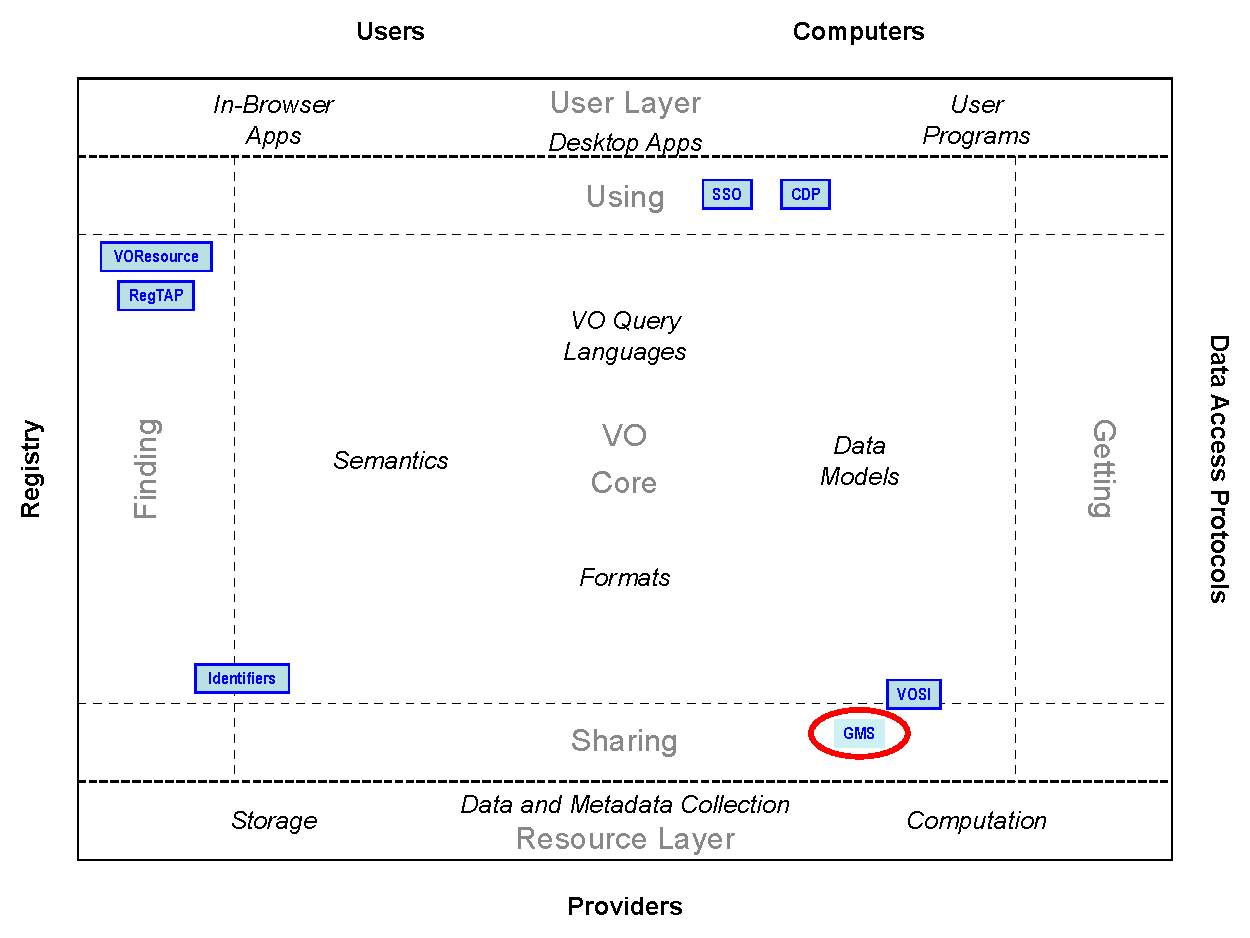
\includegraphics[width=0.9\textwidth]{role_diagram.pdf}
\caption{GMS in relation to the IVOA architecture}
\label{fig:archdiag}
\end{figure}

Fig.~\ref{fig:archdiag} shows the role this document plays within the
IVOA architecture \citep{2010ivoa.rept.1123A}.

GMS can be used by any software that needs to check, for authorization purposes, whether a user is a member of group.  Because of this general purpose functionality, GMS slices through all IVOA standards and lies in the middle of the SHARING technical resource in the IVOA architecture diagram.  Indeed, GMS allows for the sharing of proprietary resources to a limited audience.

\subsection{Scope}

When looking at a system that has proprietary resources that need to be protected, it is clear that there are two distinct phases to authorization:  the assignment of the rules protecting the resources, and the attempts by various users to gain access to those resources.  They are described here:

\begin{enumerate}
\item The owner(s) of a resource may, at any time, change the rules by which a resource may be accessed. This is the \emph{granting and revoking of access}.
\item When users try to access resources, the granting rules for that resource are evaluated at runtime. This is the \emph{authorization check}.
\end{enumerate}

GMS presents an interoperable solution for item 2, the \emph{authorization check}, though it acknowledges that step 1, \emph{granting and revoking of access} is a part of the authorization process.

\subsection{Definitions}

\paragraph{Authentication} User identification through credentials or identity provider.  Refer to the IVOA Single-Sign-On Profile: Authentication Mechanisms  \citep{2017ivoa.spec.0524T}.

\paragraph{Authorization} Making the decision of whether to grant a user permission to a given resource.  The decision usually involves knowing the user's identity obtained through authentication.

\paragraph{GMS Authorization} Making the decision of whether to grant a user permission to a given resource by ensuring the authenticated user is a member of the group assigned to protect that resource.

\paragraph{Resource} Something that may require authorization for access.  For example, a service, a data file, metadata, a catalog, or infrastructure.

\paragraph{User} An individual or entity identified by authentication that is attempting to perform some action.

\paragraph{Group} A set of users.

\paragraph{Grant} Authorizing access to a proprietary resource by assigning a group to protect that resource.

\paragraph{Revoke} Removing access to a proprietary resource by removing an assigned group.

\paragraph{Owner} A user or group of users who may grant or revoke access to a specific resource.

\subsection{Usage Scenarios}
\label{subsec:usecases}

Aside from the main use case of restricting access to proprietary resources, GMS supports a number of other use cases, of both the user and system variety.

\paragraph{Proprietary information} Restricting access to proprietary resources to certain users.

\paragraph{Homogeneity} Using the same mechanism to control access to proprietary resources in a data centre or in multiple data centres.

\paragraph{Scalability} A distributed mechanism that scales linearly with the resources being protected.

\paragraph{Remotely managing access} A project may wish to control access to resources that reside externally.

\paragraph{Access rule sharing} A project may consist of a variety of resources that can be all managed by the same access rule: group membership certification.

\paragraph{Extending the services of a data centre} A project that has hosted data and metadata at a data centre may wish to create value-added services outside of the data centre itself.  If some of the data or metadata is proprietary, the extended services may need to determine if a user is allowed to perform certain action on that data or metadata.  A remote GMS instance can be used in this way.

\paragraph{Cooperating institutes} Two or more institutes may work together on a single project that involves proprietary resources and would benefit from a single, standard mechanism for protecting those resources.

\section{Groups}

\subsection{Why Groups?}
\label{subsec:whygroups}

Why are groups a good model for authorization?  When a system needs to perform an \emph{authorization check} on a resource, it is trying to determine if the authenticated user is allowed access.  There are a number of options on how this can be accomplished.

A simple approach would be to add the identity of the user to the resource.  However, this is too restrictive as there may be multiple users who are allowed access.  So, we could instead add a list of user identities to the resource being protected.  It becomes a problem when there are two resources that need protecting by the same set of individuals.  This becomes difficult to maintain because a change in access rules (\emph{granting and revoking access}) would mean a change to multiple resources.

So, it becomes clear that this list of users needs to be decoupled from the resource so that it can be referenced and shared by multiple resources.  To do so, the list must become a single entity that can be referenced by a name.  And so, we must have a named group of users.

A central repository of groups of users would introduce other problems:  a single point of failure, and the inability to partition groups of users.  Thus, the \emph{location} of the group must accompany the group reference so that it is possible to have multiple collections of groups of users and multiple associated GMS services.

Resources must then reference a group by a URI with a location and a name that is unique within that location.  This is called the Group Identifier.

Systems must use the information in the group identifier to determine if the user is a member of the group.  Because the location may be outside of the immediate vicinity of the resource, this query must be performed in a standard and accessible manner and so is defined as a RESTful interface to group membership.

\subsection{Group Identifiers}
\label{subsec:groupids}

A \emph{group identifier} is used to uniquely and universally identify individual groups.  They are attached to proprietary resources for the purpose of referencing the group (or groups) whose members are authorized to access that resource.  When a system needs to do an authorization check because a request for access is being made, it can make the decision based on the response of a membership call to a GMS service.  By using an IVOA Registry, the system has all the information it needs within the group identifier to locate the associated GMS service and formulate the REST call to that service for the membership check.

Group identifiers are IVOA Identifiers (IVOIDs, \citet{2016ivoa.spec.0523D}).  This means they can be used to look up the underlying GMS service in an IVOA registry (as is explained in the IVOA Identifiers document).  Group names are specified in the \emph{query} part of the IVOID and are mandatory in group identifiers.  So, group identifiers must conform to all the rules of IVOIDs and also MUST include the \emph{query} part of an IVOID representing the group name.  Group names are case-sensitive and must consist only of alphanumeric characters (ASCII 65-122) and any of the following: commas, dashes, periods, underscores, and tildes (ASCII 44, 45, 46, 95, and 126 respectively).

Below is an example of a valid and typical group identifier with group name \emph{mygroup}:

\begin{verbatim}
ivo://authority.example.com/groupService?mygroup
\end{verbatim}

To obtain the access URL for a GMS service, a Registry query is performed. Using RegTAP \citep{2014ivoa.spec.1208D}, one uses the following three costraints from the \emph{interface} table:

\begin{itemize}
\item{\emph{ivoid}} - The \emph{registry part} of the group identifier.
\item{\emph{standard\_id}} - The desired search feature of GMS.
\item{\emph{intf\_role}} - Always '\emph{std}', to indicate a standard service is being queried for.
\end{itemize}

and one optional constraint, \emph{security\_method\_id}, used to identify how clients can authenticate to the GMS service.  To find a GMS service that does not require authorization, the value of the security\_method\_id constraint would be NULL.  However, since anonymously accessible GMS services are not likely to exist (see section \ref{subsec:creddel}), the query should either:

\begin{itemize}
\item include a desired security\_method\_id in the where clause, as specified by the IVOA Single-Sign-On Profile \citep{2017ivoa.spec.0524T}, or;
\item omit the constraint and iterate over the resulting rows to choose an appropriate security method.
\end{itemize}

At the time of writing, the approach the IVOA is taking to discover service authentication support is changing.  Please consult the latest version of the Single-Sign-On Profile for details.

The following query will return a row for each access\_url and security\_method\_id combination.  The ivoid value is calculated by removing the query string from the group identifier.  Since we are looking to perform an \emph{is member} call, we ask for the GMS search capability, identified by the GMS search standardID (see section \ref{subsec:api}). \footnote{To find a RegTap service on which to execute this query, consult http://rofr.ivoa.net/}

\begin{lstlisting}[language=SQL,xleftmargin=2em]
SELECT access_url, security_method_id
FROM rr.interface
NATURAL JOIN rr.capability
NATURAL JOIN rr.resource
WHERE
  ivoid = 'ivo://authority.example.com/groupService'
  AND standard_id LIKE 'ivo://ivoa.net/std/gms#search-1.%'
  AND intf_role='std'
\end{lstlisting}

This would result in one or more access URLs capable of performing a GMS search on the group 'groupName' with its corresponding security method support.  For example, it could return two rows to the same GMS instance with support for different security methods:

\vspace{3mm}
\hskip-1.0cm
\begin{tabular}{l l}
\textbf{access\_url} & \textbf{security\_method\_id} \\
\sptablerule
https://server.example.com/gms/search & ivo://ivoa.net/sso\#tls-with-certificate \\
https://server.example.com/gms/search & ivo://ivoa.net/sso\#token \\
\sptablerule
\end{tabular}
\vspace{3mm}

To then perform the group membership query on any of these URLs, the service would formulate a REST call as defined by the GMS Search API.  Since it is required that the calls be made \emph{as the user}, the call, in this example, must be made with either the user's delegated client certificate or the user's delegated authorization token with the appropriate scope.

\subsection{Caching}
\label{subsec:caching}

Clients and services that will require frequent lookups of GMS services should strongly consider caching a map of group identifier keys to access URLs values. Access URLs likely change very infrequently.  Caching will reduce the traffic on the RegTap services and improve the performance of authorization checks in general.

Group membership information from specific GMS services can also be cached.  Again, caching will improve performance, but will also add tolerance to authorization checks when GMS services are down, as clients and services can consult the cache for membership information as a backup option.  The duration in which a group membership cache should be considered valid (not stale) is the decision of the party performing the authorization check--it is most informed as to the importance of up-to-date membership information for doing authorization checks.  GMS services should, however, set the HTTP response header \emph{Expires} to an HTTP-date (see section 5.3 in RFC 7234 \citep{std:RFC7234}) indicating how long the service thinks the membership information should be considered valid.  This date can help clients choose an expiry time for group membership caches.

\section{GMS Search API}

\subsection{API Definition}
\label{subsec:api}

The Group Membership Service defines a RESTful API \citep{fielding00} that allows for the determination of whether a user is a member of a group.  This functionality is represented with the following standard ID:

\begin{verbatim}
    ivo://ivoa.net/std/gms#search-1.0
\end{verbatim}

As explained in \ref{subsec:groupids}, the combination of this standard ID and a serviceID (extracted from the group identifier) results in an \xmlel{access\_url}.

An HTTP GET to the \xmlel{access\_url} returns a list of group names in which the calling user is a member.  One or more \emph{group} query parameters may be included in the HTTP GET.  If any \emph{group} parameters are included, the search is to be limited to the union of groups identified by those parameters.  If no \emph{group} parameters are included, all groups known to the service must be checked for membership.  Thus, the inclusion of \emph{group} parameters changes (reduces) the scope of the membership search.

The value of each \emph{group} parameter is the groupName part of a Group Identifier.

For a successful HTTP GET to the search endpoint (whether \emph{group} parameters are included or not), the service shall respond with HTTP 200 (OK).  Even if the user belongs to none of the groups in the scope of the request, the service shall respond with a 200 if the membership check(s) was successful.

On a successful HTTP GET, the service must write the name of each of the groups in which the user is a member in the response body in \emph{text/plain} format.  Each group name (even the last) must end with a newline as a CRLF\footnote{Carriage Return character (ASCII 13) plus a Line Feed character (ASCII 10)}.  If the user is not a member of any groups within the scope of the search the service must return an empty response body.  The service should ignore any group names it does not recognize.

It is the authenticated user (the user making the REST call) who is the subject of the membership question.  Users' identity is determined by one of the authentication mechanisms described in the IVOA Single-Sign-On Profile.  Because GMS is most useful to services with proprietary information (ie. it is not users themselves), users' delegated credentials will be used extensively to make GMS calls.  (See section \ref{subsec:creddel} for more information.)

If the user cannot be identified from the call because they have not authenticated (the request is anonymous), the service must respond with HTTP 401 (Unauthorized).  The response message should indicate that authentication is required to use the service.

If an authenticated user could not be identified from the HTTP request the service must response with HTTP 403 (Forbidden).

\subsection {Search Examples}
\label{subsec:examples}

\paragraph{Example 1 - Group access to a VOSpace Node}

A VOSpace service receives a request from a user to read a node that has the group-read property set to

\begin{verbatim}
ivo://authority.example.com/gms/instance1?my-collaboration
\end{verbatim}

The VOSpace service resolves the Group URI to a URL hosting the associated Group Membership Service as per the steps outlined in section \ref{subsec:groupids}:

\begin{verbatim}
https://server.example.com/groupService/search
\end{verbatim}

To authorize the user, the VOSpace service queries the GMS search service using the user's delegated credentials.  Since it is only interested in the single group, the \emph{group} parameter is used:

\begin{verbatim}
https://server.example.com/gmsService/search?group=my-collaboration
\end{verbatim}

The GMS service identifies the user and determines that the user is a member of group 'my-collaboration'.  It then returns a response code of 200 (OK) with the string \emph{my-collaboration} (followed by CRLF) written to the response body.

\begin{verbatim}
my-collaboration
\end{verbatim}

After receiving this response, the VOSpace service concludes the user is a member of the group allowed to read the node and proceeds with the user's request.

If the user were not a member of 'my-collaboration', the GMS service would return 200 (OK) with an empty response body.  The VOSpace service would then conclude the user cannot read the node and return a 403 (Permission Denied).

In both cases the Content-type of the GMS response is set to 'text/plain'.

\paragraph{Example 2 - Group access to a service}

A web service is allowed to be used by members of one of two groups:

\begin{verbatim}
ivo://authority.example.com/gms/instance1?project-group-1
ivo://authority.example.com/gms/instance1?project-group-2
\end{verbatim}

When a user calls this protected service, the service authorizes use by making the following call to the associated GMS.

\begin{verbatim}
https://server.example.com/gmsService/search?
  group=project-group-1&group=project-group-2
\end{verbatim}

The service targets only the two groups as this is the only membership in which it is interested.  GMS determines that the user is a member of group=project-group-2 so returns a 200 response with a text/plain body:

\begin{verbatim}
project-group-2
\end{verbatim}

\paragraph{Example 3 - Group access to table data}

A user issues an ADQL query to a table with row-level authorization in a TAP service.  A read-group column defines which group is allowed to read that row.  The first row that is encountered with a non-null read-group has value:

\begin{verbatim}
ivo://authority.example.com/gms/instance1?my-collaboration
\end{verbatim}

In anticipation of more rows to follow, and to avoid needing to make multiple calls to GMS, the TAP service asks for all the user's group memberships when the first protected row is encountered.  This cached group information can be applied to all subsequent rows processed.  Again, the service uses the end user's delegated credentials in the search call.

\begin{verbatim}
HTTP GET to
https://server.example.com/gmsService/search
\end{verbatim}

The GMS service returns HTTP 200 and all the groups in which the calling user is a member:

\begin{verbatim}
my-collaboration
my-other-collaboration
my-third-collaboration
\end{verbatim}

The TAP service caches this group membership information for the lifetime of the request so that it can be used if necessary when checking other rows.  If a Group URI with a different \emph{authority} is encountered, the TAP service must call that GMS service too and add the list of groups from that authority to its cache.

\subsection {GMS and Credential Delegation}
\label{subsec:creddel}

User and group membership information may be considered private, so determining who is allowed to make GMS search calls is an important consideration.  This is part of the reason why the specification only allows for group membership checks to be made by the user whose membership is being checked (the 'target user').  This rule ensures that only the target user can see their group membership information.

This rule also means that the caller of GMS must use the credentials (proxy certificate, token, etc) of the target user.  Although users may themselves call GMS for membership information it is generally not very useful to them.  The target use case is for programmatic systems to call GMS for authorization checks.  So, those systems must have access to the target user's credentials.  This is accomplished through use of the IVOA Credential Delegation Protocol \citep{2010ivoa.spec.0218P}.

An alternative to this approach, which was considered, is to use privileged credentials to make GMS calls.  With this a number of problems related to the complexity of managing trust relationships arise.  Thus, such super-user credentials are not to be used for making calls to a GMS service.

\section{Registering GMS Services}

In this section, standard VO XML namespace prefixes apply, i.e.,
\xmlel{vr:} corresponds to VOResource \citep{2018ivoa.spec.0625P}
\nolinkurl{http://www.ivoa.net/xml/VOResource/v1.0}, and
\xmlel{vs:} corresponds to VODataService \citep{2010ivoa.spec.1202P}
\nolinkurl{http://www.ivoa.net/xml/VODataService/v1.1}.

Group membership services may be registered using any suitable resource type, where plain VOResource \xmlel{vr:Service} records are recommended.

GMS 1.0 resources MUST contain exactly one \xmlel{capability} element with a standard id of \nolinkurl{ivo://ivoa.net/std/gms#search-1.0}.  More capabilities with other or no standard ids are allowed.

This capability MUST contain one or more interface(s) of type \xmlel{vs:ParamHTTP} and a \xmlel{role} attribute set to \verb|std|, the \xmlel{accessURL} of which declare the GMS search endpoint as defined in the present document.  As dicussed in sect.~\ref{subsec:creddel}, such interfaces will in general define a \xmlel{securityMethod}.  When a service supports multiple authentication methods, it has to include multiple \xmlel{interface} elements.

Declaring other interfaces in the \verb|gms#search| capability is discouraged for interoperability; no such additional interface may declare a \xmlel{role} of \verb|std|.  Services wishing to declare non-GMS interfaces (e.g., for use with non-VO standards) should do so in separate \xmlel{capability} elements.

This way of registering enables the service discovery pattern discussed in sect.~\ref{subsec:groupids}.  A sample registry record is distributed with this specification\footnote{\auxiliaryurl{sample-record.xml}}.


\section {Implementation}

\subsection {Implementation Options}
\label{subsec:implopts}

An implementation of GMS requires a system that associates users with zero or more groups, some options include:

\begin{itemize}
\item Grouper\footnote{https://www.internet2.edu/products-services/trust-identity/grouper/} (groups in MySQL\footnote{https://mysql.com}, users in LDAP\footnote{Lightweight Directory Access Protocol})
\item By using LDAP only (some implementations require plugins to support groups)
\item Through a relational database.
\item A VOSpace implementation: It is conceivable that VOSpace could be used to implement GMS, where ContainerNodes represent groups and DataNodes represent users.
\end{itemize}

\subsection{Groups of Groups}
\label{subsec:groupsofgroups}

It may be functionally attractive to support groups within groups.  If this is implemented, then the service must ensure that this representation is reflected by the GMS service API.  For example, consider the situation where a user is a member of group G2 and group G2 is a member of group G1.  On a membership call to group G1 made by this user, the service must respond with group G1 (meaning yes: the user is a member of group G1).  The fact that the service supports groups within groups is not exposed through the search API, but the API does not prohibit such an implementation.  If the call was a memberhip check to group G2, the service would respond with G2 in the response body.

If one of the contained groups exists at another GMS instance, perhaps outside of the organization, then the service may transitively query that service to determine group membership, taking care to avoid a loop caused by groups being members of each other.

\subsection{Group Name Reuse}
\label{subsec:groupnamereuse}

GMS Services should not allow group name reuse as there is a danger of inadvertently granting access to the members of a reused group.  For instance, if an active group is used to protect a number of resources, it means that those resources reference the group URI.  If the associated group is deleted and then recreated with a new set of members, and if the remote group references are still in place, the new members will inherit access to those resources.  Thus, it is recommended that group names are never resused as it is impossible to discover from where the group has referneces.

\appendix

\section{Changes from Previous Versions}
\label{sec:changehistory}

\subsection{Changes from PR-1.0-20210609}

\begin{itemize}
\item Adding a section on how to register GMS services.
\end{itemize}

\subsection{Changes from WD-GMS-1.0-20200210}
\begin{itemize}
\item{API modification: groups identified by query parameter, not path element}
\item{API modification: multiple group parameters to allow clients to minimize required GMS calls}
\item{Update examples to match API changes}
\end{itemize}

\subsection{Changes from WD-GMS-1.0-20190506}
\begin{itemize}
\item{General text changes for clarification in abstract and document body}
\item{Removed support for identifying the 'target user' of a GMS call with id parameters.  The 'target user' is now always the user making the API call to GMS.}
\item{Added new sub-section: GMS and Credential Delegation}
\item{Section 'Authorization Requirements' renamed to 'Scope'}
\item{Section 'Use Cases' renamed to 'Usage Scenarios'}
\end{itemize}

\subsection{Changes from WD-GMS-1.0-20190329}
\begin{itemize}
\item{Reverted Group Identifier to be an IVOID}
\item{Corrected, expanded, and clarified the group identifier registry resolution procedure}
\item{Updated bibliography references}
\end{itemize}

\subsection{Changes from WD-GMS-1.0-20181025}
\begin{itemize}
\item{Changed Group identifier URI to be in the format gms://authority/path?group}
\item{Changed names of params user and principal to identity and identityType}
\item{Corrected API definition to always return 200 on succcess}
\item{REST API now described in a table}
\end{itemize}

% these would be subsections "Changes from v. WD-..."
% Use itemize environments.

\bibliography{ivoatex/ivoabib,ivoatex/docrepo}

\end{document}
